\documentclass[unicode,11pt,a4paper,oneside,numbers=endperiod,openany]{scrartcl}
\usepackage{xcolor}
\usepackage{listings}
\usepackage{amsmath}

% Define custom verbatim environment with gray background
\lstnewenvironment{grayverbatim}{%
  \lstset{backgroundcolor=\color{gray!10}, % Adjust the shade of gray as desired
          frame=single,
          framerule=0pt,
          basicstyle=\ttfamily,
          breaklines=true,
          columns=fullflexible}
}{}

\lstnewenvironment{cppverbatim}{%
  \lstset{language=C++, % Set the language to C++
          backgroundcolor=\color{gray!10}, % Adjust the shade of gray as desired
          frame=single,
          framerule=0pt,
          basicstyle=\ttfamily,
          keywordstyle=\color{blue}, % Set the color for keywords
          commentstyle=\color{green!50!black}, % Set the color for comments
          stringstyle=\color{red}, % Set the color for strings
          breaklines=true,
          showstringspaces=false, % Don't show spaces within strings
          columns=fullflexible}
}{}

\usepackage{ifthen}
\usepackage[utf8]{inputenc}
\usepackage{graphics}
\usepackage{graphicx}
\usepackage{hyperref}

\pagestyle{plain}
\voffset -5mm
\oddsidemargin  0mm
\evensidemargin -11mm
\marginparwidth 2cm
\marginparsep 0pt
\topmargin 0mm
\headheight 0pt
\headsep 0pt
\topskip 0pt        
\textheight 255mm
\textwidth 165mm

\newcommand{\duedate} {}
\newcommand{\setduedate}[1]{%
\renewcommand\duedate {Due date:~ #1}}
\newcommand\isassignment {false}
\newcommand{\setassignment}{\renewcommand\isassignment {true}}
\newcommand{\ifassignment}[1]{\ifthenelse{\boolean{\isassignment}}{#1}{}}
\newcommand{\ifnotassignment}[1]{\ifthenelse{\boolean{\isassignment}}{}{#1}}

\newcommand{\assignmentpolicy}{
\begin{table}[h]
\begin{center}
\scalebox{0.8} {%
\begin{tabular}{|p{0.02cm}p{16cm}|}
\hline
&\\
\multicolumn{2}{|c|}{\Large\textbf{HPC Lab for CSE 2024 ---  Submission Instructions}}\\
\multicolumn{2}{|c|}{\large\textbf{(Please, notice that following instructions are mandatory: }}\\
\multicolumn{2}{|c|}{\large\textbf{submissions that don't comply with, won't be considered)}}\\
&\\
\textbullet & Assignments must be submitted to \href{https://moodle-app2.let.ethz.ch/course/view.php?id=22516}{Moodle} (i.e. in electronic format).\\
\textbullet & Provide both executable package and sources (e.g. C/C++ files, Matlab). 
If you are using libraries, please add them in the file. Sources must be organized in directories called:\\
\multicolumn{2}{|c|}{\textit{Project\_number\_lastname\_firstname}}\\
& and  the  file must be called:\\
\multicolumn{2}{|c|}{\textit{project\_number\_lastname\_firstname.zip}}\\
\multicolumn{2}{|c|}{\textit{project\_number\_lastname\_firstname.pdf}}\\
\textbullet &  The TAs will grade your project by reviewing your project write-up, and looking at the implementation 
                 you attempted, and benchmarking your code's performance.\\

\textbullet & You are allowed to discuss all questions with anyone you like; however: (i) your submission must list anyone you discussed problems with and (ii) you must write up your submission independently.\\
\hline
\end{tabular}
}
\end{center}
\end{table}
}
\newcommand{\punkte}[1]{\hspace{1ex}\emph{\mdseries\hfill(#1~\ifcase#1{Points}\or{Points}\else{Points}\fi)}}


\newcommand\serieheader[6]{
\thispagestyle{empty}%
\begin{flushleft}

\includegraphics[width=0.4\textwidth]{ETHlogo_13}
\end{flushleft}
  \noindent%
  {\large\ignorespaces{\textbf{#1}}\hspace{\fill}\ignorespaces{ \textbf{#2}}}\\ \\%
  {\large\ignorespaces #3 \hspace{\fill}\ignorespaces #4}\\
  \noindent%
  \bigskip
  \hrule\par\bigskip\noindent%
  \bigskip {\ignorespaces {\Large{\textbf{#5}}}
  \hspace{\fill}\ignorespaces \large \ifthenelse{\boolean{\isassignment}}{\duedate}{#6}}
  \hrule\par\bigskip\noindent%  \linebreak
 }

\makeatletter
\def\enumerateMod{\ifnum \@enumdepth >3 \@toodeep\else
      \advance\@enumdepth \@ne
      \edef\@enumctr{enum\romannumeral\the\@enumdepth}\list
      {\csname label\@enumctr\endcsname}{\usecounter
        {\@enumctr}%%%? the following differs from "enumerate"
	\topsep0pt%
	\partopsep0pt%
	\itemsep0pt%
	\def\makelabel##1{\hss\llap{##1}}}\fi}
\let\endenumerateMod =\endlist
\makeatother




\usepackage{textcomp}





\begin{document}


\setassignment
\setduedate{11 March 2024, 23:59}

\serieheader{High-Performance Computing Lab for CSE}{2024}
            {Student: CARLA JUDITH LOPEZ ZURITA}
            {Discussed with: YANNICK RAMIC \\
            \hspace*{370pt}ALITZEL MACIAS}
{Solution for Project 1}{}
\newline

The aim of this project is to familiarize the students with the Euler cluster and to provide an
introduction to performance characteristics, memory hierarchies, and optimization techniques. The
project is divided into four sections: Euler warm-up, performance characteristics, auto-vectorization,
and matrix multiplication optimization.

\section{Euler warm-up [10 points]}

The first section is designed to familiarize the user with the basic components of the Euler cluster
available to the students and collaborators of ETH. The questions and answers are designed to
provide a brief overview of the Euler cluster and its intended function.

\begin{enumerate}

    \item \textit{What is the module system and how do you use it?}
    Modules are used to configure the environment for a particular software version.
    They configure the necesary variables to make sure all required binaries and libraries are found. 
    On the Euler cluster, there are two types of Modules packages:
    \begin{enumerate}
        \item LMOD Modules
        \item Environment Modules 
    \end{enumerate}
    To use the modules, on the terminal we write the keyword \textbf{module} followed by the commands.
    For example, to activate the LMOD module and install certain libraries or specify the version,
    run on the terminal the following commands, 
    \begin{grayverbatim}
module load gcc/6.3.0 python/3.8.5
    \end{grayverbatim}

    \item \textit{What is Slurm and its intended function?}
    Euler uses Slurm, which stands to Simple Linux Utility for Resource Management, for job management.
    In order to actually run something, for example a C++ program, the computations must be
    submitted to the batch system. To submit scripts to Slurm use the following line,
    \begin{grayverbatim}
sbatch [options] --wrap "command [arguments]"
    \end{grayverbatim}
    Basically, instead of running an executable using the command \textbf{./a.out}, one would run 
    \begin{grayverbatim}
sbatch --wrap "./a.out"
    \end{grayverbatim}
    To see the job list, run \textbf{squeue}. You can also cancel your job with \textbf{scancel} 
    plus the job number.
    To avoid writing the sequence of commands manually and to add more flags or specifications, 
    you can use a batch script, whcih can be then run using,
    \begin{grayverbatim}
sbatch < my_batch_script.sh
    \end{grayverbatim}

    \item \textit{Write a simple “Hello World” C/C++ program which prints the host name of the 
    machine on which the program is running. }
    Attached bellow is a C++ program for getting the hostname. 
    I tried using the $<$limits.h$>$ header file but I couldn't retrieve HOST\_NAME\_MAX (using the C++ compiler on macOs).
    \begin{cppverbatim}
#include <iostream>
#include <unistd.h> // For gethostname function

int main()
{
char hostname[256]; // Guess for size of hostname

// Get the host name
if (gethostname(hostname, sizeof(hostname)) == 0)
{
    // Success
    std::cout << "Hello world, this program is running on" 
    << hostname << std::endl;
}
else
{
    // Error
    std::cerr << "Failed to get the host name" << std::endl;
}

return 0;
}
    \end{cppverbatim}
    The output when running this small program was: 
    \begin{grayverbatim}
Hello world, this program is running on Carlas-MacBook-Pro.local
    \end{grayverbatim}
    
    \item \textit{Write a batch script which runs your program on one node. The batch script should
    be able to target nodes with specific CPUs.
    Hint: Slurm has the option --constraint to select some nodes with specific features. Possible
    options to select nodes featuring a certain CPU: EPYC\_7742, EPYC\_7H12, EPYC\_7763, EPYC\_9654.}

    We can use the help of the page \href{https://scicomp.ethz.ch/public/lsla/index2.html}{LSF/Slurm Submission Line Advisor}
    to write the batch script. For this exercise, I used the skeleton source priveded in the class material.
    The output was two files, an \textit{out} file and an \textit{err} file, both named
    \textit{slurm\_job\_one-48720143}. The \textit{out} file contained the following info,
    \begin{grayverbatim}
Model name:            AMD EPYC 9654 96-Core Processor
eu-g9-046-1
    \end{grayverbatim}    


    \item \textit{Write another batch script which runs your program on two nodes. Check that the
    Slurm output file slurm.out by default contains two different host names}
    Once again, I used the template provided in the Moodle of the course and again obtained
    two files (\textit{out} and \textit{err}), this time named \textit{slurm\_job\_two-48756918}. The \textit{out} file reads,
    \begin{grayverbatim}
Model name:            AMD EPYC 7763 64-Core Processor
eu-a2p-381
eu-a2p-385
    \end{grayverbatim}    


\end{enumerate}

\section{Performance characteristics [50 points]}
In order to understand the performance characteristics of a computing system, we need to
know what physical constraints limit data transfer rates and computation speeds within it.
In this section, we will analyze the peak performance of the Euler VII (Phase I and II) clusters,
the memory hierarchies, and the STREAM benchmark. We will also use the roofline model to analyze the
performance of the nodes.

\subsection{Peak performance}\label{sec:peak_performance}
In this task, we compute the peak performance of a core, CPU, node and cluster for the Euler VII
(Phase I and II) nodes. The peak performance $P$ of each of the elements is computed as follows
\begin{center}
    $P_{core}  = n_{super} \times n_{\tiny{\textrm{FMA}}} \times n_{\tiny{\textrm{SIMD}}} \times f$,
\end{center}
\begin{center}
    $P_{CPU} = n_{cores} \times P_{core}$,
\end{center}
\begin{center}
    $P_{node} = n_{sockets} \times P_{CPU}$,
\end{center}
\begin{center}
    $P_{cluster} = n_{nodes} \times P_{node}$,
\end{center}
where $n_{\tiny{\textrm{super}}}$ is the superscalarity factor, $n_{\tiny{\textrm{FMA}}}$ is the fused 
multiply-add factor, $n_{\tiny{\textrm{SIMD}}}$ is the SIMD (Single Instruction, Multiple Data) factor,
and $f$ is the (base) clock frequency. $n_{cores}$ is the number of cores per CPU, $n_{sockets}$ is the 
number of sockets per node, and $n_{nodes}$ is the number of nodes in the cluster.

For Phase I, we find the corresponding values in the literature and resources available online.
\begin{itemize}
    \item $n_{\tiny{\textrm{super}}}$: 2 \cite{uops-info}
    \item $n_{\tiny{\textrm{FMA}}}$: 2 \cite{uops-info}
    \item $n_{\tiny{\textrm{SIMD}}}$: SIMD width supported by AMD Zen2 is 256 bits per SIMD register. 
    % This means that the CPU can process up to 8 single-precision (float32) or 4 double-precision (float64).
     \cite{hager2021amd}
    \item $f$: 2.6 GHz nominal, 3.3 GHz peak \cite{euler-ethz}
    \item $n_{cores}$: 64-core AMD EPYC 7H12 processors per CPU (Product Line: AMD EPYC™ 7002 Series) \cite{amd-epyc-7H12}
    \item $n_{sockets}$: each node has 2 AMD EPYC 7H12 CPUs \cite{euler-ethz}
    \item $n_{nodes}$: 292 compute nodes — HPE ProLiant XL225n Gen10 Plus \cite{euler-ethz}
\end{itemize}
The peak performance is computed as follows
\begin{center}
    $P_{core}  = 2 \times 2 \times 4 \times 2.6 \textrm{ GHz}= 41.6 \textrm{ GFlops/s}$
\end{center}
\begin{center}
    $P_{CPU} = 64 \times 41.6 = 2662.4 \textrm{ GFlops/s}$
\end{center}
\begin{center}
    $P_{node} = 2 \times 2662.4 = 5324.8 \textrm{ GFlops/s}$
\end{center}
\begin{center}
    $\boxed{P_{\textrm{Euler VII.I}} = 292 \times 5.325 \textrm{ TFlops/s}  = 1,554.8416 \textrm{ TFlops/s}}$
\end{center}

For Phase II:
\begin{itemize}
    \item $n_{\tiny{\textrm{super}}}$: 2 \cite{uops-info}
    \item $n_{\tiny{\textrm{FMA}}}$: 2 \cite{uops-info}
    \item $n_{\tiny{\textrm{SIMD}}}$: 4 double-precision (AMD Zen3) \cite{hager2021amd}
    \item $f$: 2.45 GHz nominal, 3.5 GHz peak \cite{euler-ethz}
    \item $n_{cores}$: 64-core AMD EPYC 7763 processors per CPU (Product Line: AMD EPYC™ 7003 Series) 
        \cite{amd-epyc-7763}
    \item $n_{sockets}$: each node has 2 AMD EPYC 7763 CPUs \cite{euler-ethz}
    \item $n_{nodes}$: 248 compute nodes — HPE ProLiant XL225n Gen10 Plus \cite{euler-ethz}
\end{itemize}
The peak performance is computed as follows
\begin{center}
    $P_{core}  = 2 \times 2 \times 4 \times 2.45 \textrm{ GHz}= 39.2 \textrm{ GFlops/s}$
\end{center}
\begin{center}
    $P_{CPU} = 64 \times 39.2 = 2508.8 \textrm{ GFlops/s}$
\end{center}
\begin{center}
    $P_{node} = 2 \times 2508.8 = 5017.6 \textrm{ GFlops/s}$
\end{center}
\begin{center}
    $\boxed{P_{\textrm{Euler VII.II}} = 248 \times 5.018 \textrm{ TFlops/s}  = 1,244.365 \textrm{ TFlops/s}}$
\end{center}

From the calculatiosn, we can see that the peak performance of the Euler VII (Phase I) cluster is greater than
the peak performance of the Euler VII (Phase II) cluster. This is due to the higher base and peak clock frequency
of the AMD EPYC 7H12 processor compared to the AMD EPYC 7763 processor.

\subsection{Memory Hierarchies}
The memory hierarchy of a computing system is a pyramid of storage devices with different capacities,
access times, and costs. In this section, we identify the parameters of the memory hierarchy on a node
of the Euler VII (Phase I and II) cluster.

\subsubsection{Cache and main memory size}
After logging into the Euler VII (Phase I and II) cluster, we can use the \textbf{lscpu} command to obtain information
about the CPU architecture. We also read the file \textbf{/proc/meminfo} to obtain information about the main memory.
Finally, \textbf{hwloc-ls} can be used to obtain information about the cache sizes. The results are shown in Table \ref{tab:memory_config}.
Each core has its own L1 and L2 cache. The retrived information reveals that the L3 cache is shared among eight 
cores for the AMD EPYC 7H12 and four cores for the AMD EPYC 7763. 
The schemas of the memory hierarchy of both processors can be found in 
Figure \ref{fig:7H12_processor} and Figure \ref{fig:7763_processor} included in the Appendix.


\begin{table}[h]
    \centering
    \caption{Memory hierarchy of Euler VII login nodes Phases I and II.}
    \begin{tabular}{||c c c||} 
     \hline
    Euler VII & Phase I & Phase II \\ [0.5ex] 
    CPU & AMD EPYC 7H12 & AMD EPYC 7763 \\
    \hline\hline
     Main memory & 31 GB & 31 GB \\ 
     \hline
     L3 cache & 16 MB & 32 MB \\
     \hline
     L2 cache & 512 KB & 512 KB \\
     \hline
     L1d cache & 32 KB & 32 KB \\
     \hline
     L1i cache & 32 KB & 32 KB \\
     \hline
    \end{tabular}
    \label{tab:memory_config}
\end{table}


\subsection{Bandwidth: STREAM benchmark}\label{sec:STREAM_benchmark}
We now consider in our analysis th speed of the memory system, quantitatively measured using its 
bandwith, which can be obtained using the STREAM benchmark. STREAM uses four different kernels (or 
operations) to measure the sustainable memory bandwidth of a system and its corresponding
computation rate. These kernels are:
\begin{itemize}
    \item \textbf{Copy}: Copying elements from one array to another.
    \item \textbf{Scale}: Multiplying each element of an array by a scalar.
    \item \textbf{Add}: Adding elements of two arrays and storing the result in a third array.
    \item \textbf{Triad}: Combining the scale and add operations.
\end{itemize}

The STREAM benchmark for Euler VII Phase I (AMD EPYC 7H12) was executed with the following parameters:
\begin{itemize}
    \item Array size: 8,500,000 elements
    \item Offset: 0 elements
    \item Memory per array: 64.8 MiB (= 0.1 GiB)
    \item Total memory required: 194.5 MiB (= 0.2 GiB)
    \item Each kernel was executed 20 times
\end{itemize}

The results of the analysis are shown in Table \ref{tab:performance_I}. 
We observe that the bandwidths resulting from the Scale, Add, and Triad kernels are roughly
consistent, while the bandwidth for the Copy kernel appears to be substantially higher. 
For a rough estimate, we can assume a maximum bandwidth \textbf{bSTREAM = 27 GB/s}.
\begin{table}[htbp]
    \centering
    \caption{Performance Metrics for Euler VII Phase I (AMD EPYC 7H12).}
    \begin{tabular}{||lcccc||}
        \hline
        Function & Best Rate (MB/s) & Avg time (s) & Min time (s) & Max time (s)\\
        \hline
        \hline
        Copy    & 38822.9 & 0.003888 & 0.003503 & 0.004435 \\
        \hline
        Scale   & 29254.1 & 0.005408 & 0.004649 & 0.005897 \\
        \hline
        Add     & 27327.9 & 0.008317 & 0.007465 & 0.009960 \\
        \hline
        Triad   & 27991.3 & 0.008281 & 0.007288 & 0.010853 \\
        \hline
    \end{tabular}
    \label{tab:performance_I}
\end{table}

The STREAM benchmark for Euler VII Phase II (AMD EPYC 7763) was executed with the following parameters:
\begin{itemize}
    \item Array size: 17,000,000 elements
    \item Offset: 0 elements
    \item Memory per array: 129.7 MiB (= 0.1 GiB)
    \item Total memory required: 389.1 MiB (= 0.4 GiB)
    \item Each kernel was executed 20 times
\end{itemize}

The results of the analysis are shown in Table \ref{tab:performance_II}.
We observe that the bandwidths resulting from the Scale, Add, and Triad kernels are roughly
consistent, while the bandwidth for the Copy kernel appears to be substantially higher. 
For a rough estimate, we can assume a maximum bandwidth \textbf{bSTREAM = 34 GB/s}.
\begin{table}[htbp]
    \centering
    \caption{Performance Metrics for Euler VII Phase II (AMD EPYC 7763).}
    \begin{tabular}{||lcccc||}
        \hline
        Function & Best Rate (MB/s) & Avg time (s) & Min time (s) & Max time (s)\\
        \hline
        \hline
        Copy    & 45822.8 & 0.006177 & 0.005936 & 0.006613 \\
        \hline
        Scale   & 34862.8 & 0.008157 & 0.007802 & 0.009234 \\
        \hline
        Add     & 33923.6 & 0.012687 & 0.012027 & 0.015450 \\
        \hline
        Triad   & 33951.9 & 0.012721 & 0.012017 & 0.014769 \\
        \hline
    \end{tabular}
    \label{tab:performance_II}
\end{table}

\subsection{Performance model: A simple roofline model}
The roofline model offers valuable insights into a system's performance characteristics by graphing achievable
performance against the operational intensity of a kernel. Operational intensity, defined as the
ratio of floating-point operations to bytes transferred from memory, guides this analysis.

The model delineates two key regions: memory-bound and compute-bound. In the memory-bound segment,
performance is constrained by the system's memory bandwidth, whereas the compute-bound area is
limited by the processor's peak computational capacity. This is useful for identifying performance
bottlenecks within the system.

We present the roofline models for single cores of Euler VII (Phases I 
and II) nodes, as well as the roofline model for Euler III, presented in class, for reference 
purposes. 
The model was calculated using the values for the peak performance ($P_{\text{Peak}}$) 
presented in Section \ref{sec:peak_performance} and the memory bandwidths ($b_{\text{STREAM}}$) found in
Section \ref{sec:STREAM_benchmark}.
We can identify the ridge point of the roofline model, which represents the transition point between
the memory-bound and compute-bound regions in terms of its operational intensity $I_{\text{ridge}}$. 
Table \ref{tab:ridge_point} summarizes these three values for the Euler III and Euler VII (Phase I and II) cores.
\begin{table}[htbp]
    \centering
    \caption{Peak performance ($P_{\text{Peak}}$), memory bandwith ($b_{\text{STREAM}}$) and ridge point ($I_{\text{ridge}}$)
    for different Euler cores.}
    \begin{tabular}{||lccc||}
        \hline
        Core & $P_{\text{Peak}}$ & $b_{\text{STREAM}}$ & $I_{\text{ridge}}$ \\
        \hline
        \hline
        Euler VII (Phase I) & 41.6  (GFlops/s) & 27 (GB/s) & 1.5407 (Flops/B) \\
        Euler VII (Phase II) & 39.2 (GFlops/s)  & 34 (GB/s) & 1.1529 (Flops/B) \\
        Euler III & 48 (GFlops/s)  & 12 (GB/s) & 4.0000 (Flops/B) \\
        \hline
    \end{tabular}\label{tab:ridge_point}
\end{table}
The results are shown in Figure \ref{fig:roofline}.
\begin{figure}[htbp]
    \centering
    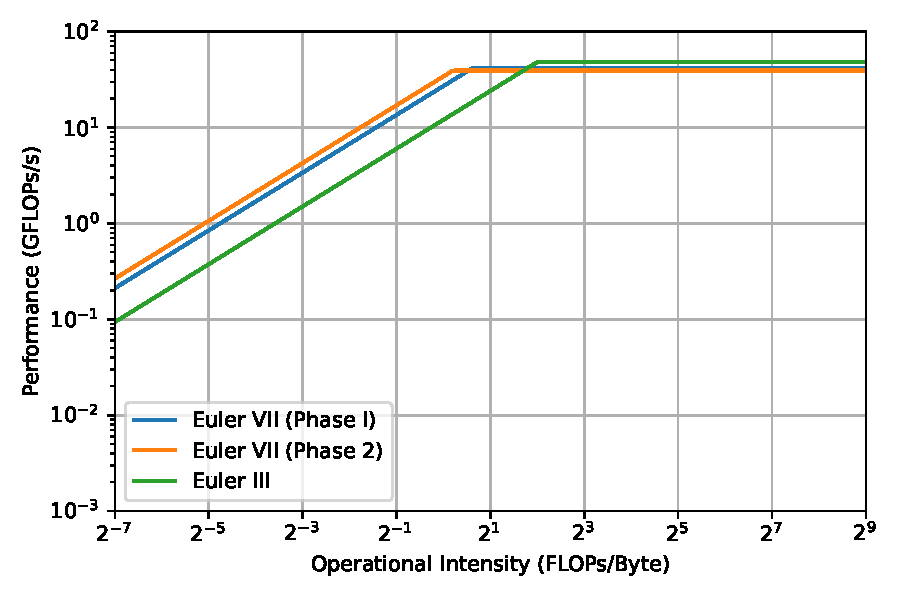
\includegraphics[width=0.8\textwidth]{../roofline/roofline.pdf}
    \caption{Log-Log Roofline Model for Euler III and Euler VII Nodes (Phase I and II).}
    \label{fig:roofline}
\end{figure}

\section{Auto-vectorization [10 points]}

After reading the Chapter “Automatic Vectorization” of the \textit{Intel oneAPI DPC++/C++ Compiler Developer
Guide and Reference} \cite{intel-oneapi}, we provide a brief answer to the following questions:

\begin{enumerate}
    \item \textit{Why is it important for data structures to be aligned?}
    Data structure alignment referts to the organization and retrieval of data stored in memory.
    It involves adjusting data objects in relation to each other.
    For example, the Intel oneAPI DPC++/C++ compiler can arrange variables to begin at specific
    memory addresses, improving memory access speed.
    Misaligned memory accesses may result in significant performance declines on certain processors
    that lack hardware support for them.

    \item \textit{What are some obstacles that can prevent automatic vectorization by the compiler?}
    Some obstacles that may cause the compiler not to vectorize include non-conntiguous memory access and
    data dependencies.
    Non-contiguous memory access occurs when the data is not stored in a contiguous block of memory and
    therefore leads to inneficcient memory access. The most prominent examples are loops with non-unit
    stride or indirect addressing.
    On the other hand, data dependencies occur when the result of changing the order of operations
    necessary for vectorization would change the result of the program. This can be caused by 
    loop-carried dependencies, anti-dependencies, and output dependencies.

    \item \textit{Is there a way to help the compiler to vectorize and how?}
    Sometimes, the compiler is unsure as to whether or not it is safe to vectorize a loop.
    You can help the compiler vectorize by the use of pragmas, keywords and options/switches.

    Pragma directives are used to provide additional information to the compiler about how to optimize the code.
    For example, whether it is safe to ignore any potential data dependencies, give hints about the loop structure,
    ask the compiler to vectorize or nor certain loops, assert that the data is aligned, and many others.

    Certain keywords can help the compiler with optimization. 
    Specifically, the \textit{restrict} keyword can be used to tell the compiler that the pointer is the only
    pointer that can access the data it points to.
    It is similar to the \textit{const} keyword, but for pointers, and the pragma \textit{ivdep}.
    The drawback is that not all compilers support keywords, which reduces portability.

    Finally, options/switches can be used to enable different levels of optimizations, such as 
    Interprocedural Optimization (IPO) and High-Level Optimizations (HLO).

    \item \textit{Which loop optimizations are performed by the compiler to vectorize and pipeline loops?}
    Loop vectorization transforms scalar loops into vectorized loops that can process multiple data elements 
    in parallel using SIMD (Single Instruction, Multiple Data) instructions. This optimization can significantly
    improve performance by utilizing the full power of vectorized hardware.

    In order to efficienly vectorrize loops, the compiler does some optimizations automatically, such as 
    loop unrolling, loop fusion, loop interchange, and loop sectioning (also known as stip-mining). 
    Loop unrolling means that the compiler replicates the loop body. 
    Loop fusion combines multiple loops into a single loop, 
    while loop interchange changes the order of nested loops. 
    Loop sectioning divides a loop into smaller blocks.
    All of these techniques aim to reduce loop overhead and improve data temporal and spatial locality, 
    allowing the process of vectorization to be more efficient.
    
    \item \textit{What can be done if automatic vectorization by the compiler fails or is sub-optimal?}
    
    There are a number of strategies that can be used in case automatic vectorization by the compiler fails or is sub-optimal.
    Manual vectorization involves using explicit vector programming models, such as SIMD intrinsics or 
    compiler-specific vectorization directives.
    You can also try restructuring the code to improve data locality and reduce data dependencies, for example try
    different data structures such as structures of arrays instead of arrays of structures as was discussed in the chapter.
    YOu can also try vector blocking, which is a technique that divides the data into smaller blocks that fit into the cache.
    Finally, you can use profiling tools and performance analysis to identify vectorization bottlenecks and understand
    where the issue might be. Trying out differente compiler flags and options can also help.

\end{enumerate}
\section{Matrix multiplication optimization [30 points]}
% Implementation: Implement blocking for square matrix multiplication in dgemm\_blocked.c.
In this section, we implemented the matrix-matrix multiplication using three algorithms, the naive approcah
the blocked algorithm, and using the OpenBLAS library when running it on an \textbf{AMD EPYC\_7763 CPU}. 
Afterwards, we optimized the blocked algorithm to maximize its performance using different techniques and 
strategies that will be discussed in the following paragraphs. We use the OpenBLAS implementation as 
benchmark, and can be also refered to in the text as \textit{reference}.

The routines perform a \textit{dgemm} operation, $C := C + A * B$
where $A$, $B$, and $C$ are lda-by-lda matrices stored in column-major format.
On exit, $A$ and $B$ maintain their input values. The implementation of the naive approach is shown in the following code snippet.
\begin{cppverbatim}
const char *dgemm_desc = "Naive, three-loop dgemm.";

void square_dgemm(int n, double *A, double *B, double *C)
{
  for (int i = 0; i < n; ++i)
  {
    for (int j = 0; j < n; ++j)
    {
      for (int k = 0; k < n; ++k)
      {
        C[i + j * n] += A[i + k * n] * B[k + j * n];
      }
    }
  }
}

\end{cppverbatim}
Similarly, the implementation of the blocked algorithm is shown in the following code snippet.
The L1 cache size for the AMD EPYC 7763 is 52 KB, which can be written down using the bitwise
left shift operator. The block size is calculated as $s = \sqrt{M/ 3}$, which is then
used to divide the matrix into blocks of size $s \times s$. Finally, the macro-kernel
is used to perform the multiplication of the blocks.
\begin{cppverbatim}
const char *dgemm_desc = "Blocked dgemm.";
#include <math.h>

void square_dgemm(int n, double *A, double *B, double *C)
{
  const unsigned int L1 = 1 << 15;                                   // L1 cache size 52 KB
  unsigned int n_ = (unsigned int)sqrt(L1 / (3.0 * sizeof(double))); // block size

  for (unsigned int j = 0; j < n; j += n_)
  {
    for (unsigned int k = 0; k < n; k += n_)
    {
      for (unsigned int i = 0; i < n; i += n_)
      {
        // Macro-kernel
        for (unsigned int jj = j; jj < (j + n_ > n ? n : j + n_); ++jj)
        {
          for (unsigned int kk = k; kk < (k + n_ > n ? n : k + n_); ++kk)
          {
            double b = B[kk + jj * n];
            for (unsigned int ii = i; ii < (i + n_ > n ? n : i + n_); ++ii)
            {
              C[ii + jj * n] += A[ii + kk * n] * b;
            }
          }
        }
      }
    }
  }
}

\end{cppverbatim}

% Optimization: Optimize your code to maximize its performance. Consider various strategies, such
% as compiler options, tuning data access patterns (including block size adjustments), using \#pragma
% directives, vectorization, loop unrolling, and more.
The summary of the results of the performance of the three algorithms using no compilation flags 
is shown in Table \ref{tab:performance_summary_base}.
\begin{table}[htbp]
    \centering
    \caption{Performance summary using no compilation flags.}
    \begin{tabular}{||lcc||}
        \hline
        Algorithm & Avg Gflop/s & Avg Percentage \\
        \hline
        \hline
        Naive, three-loop dgemm & 0.37 & 1.16\% \\
        Reference dgemm & 40.65 & 105.61\% \\
        Blocked dgemm & 0.54 & 1.37\% \\
        \hline
    \end{tabular}\label{tab:performance_summary_base}
\end{table}
Afterwards, we tried several compiler flags to optimize the performance of both the naive and 
the blocked algorithms. The compiler flags added were:
\begin{grayverbatim}
-march=native -mtune=native -ffast-math -funroll-loops -ftree-vectorize -fopenmp
\end{grayverbatim}
The compiler flags \textbf{-march=native} and \textbf{-mtune=native} optimize code generation for the host
machine's CPU architecture, leveraging its specific instruction set and tuning parameters
for performance. The \textbf{-ffast-math} flag enables aggressive optimizations on floating-point
arithmetic, potentially sacrificing strict IEEE compliance for speed. With \textbf{-funroll-loops},
the compiler replicates loop bodies to reduce loop overhead and increase parallelism.
\textbf{-ftree-vectorize} automatically transforms scalar operations into SIMD instructions, enhancing
performance on SIMD architectures. Finally, \textbf{-fopenmp} enables OpenMP support, allowing developers
to parallelize code easily for multi-core processors. Together, these flags streamline code
execution and leverage hardware capabilities to maximize performance.
The results of the performance of the three algorithms using these compilation flags is 
described in Table \ref{tab:performance_summary_some}.
\begin{table}[htbp]
    \centering
    \caption{Performance summary using some compilation flags.}
    \begin{tabular}{||lcc||}
        \hline
        Algorithm & Avg Gflop/s & Avg Percentage \\
        \hline
        \hline
        Naive, three-loop dgemm & 0.46 & 1.16\% \\
        Reference dgemm & 40.96 & 101.91\% \\
        Blocked dgemm & 0.53 & 1.35\% \\
        \hline
    \end{tabular}\label{tab:performance_summary_some}
\end{table}
From the results, we can see that the performance of the naive algorithm improved slightly
but the blocked algorithm remained the same. 
We then tried adding the \textbf{-O3} flag, which is the highest stable (or trusted) optimization level,
to the already discussed flags. 
The results are shown in Table \ref{tab:performance_summary_O3}.
\begin{table}[htbp]
    \centering
    \caption{Performance summary using -O3 compilation flag.}
    \begin{tabular}{||lcc||}
        \hline
        Algorithm & Avg Gflop/s & Avg Percentage \\
        \hline
        \hline
        Naive, three-loop dgemm & 2.08 & 5.08\% \\
        Reference dgemm & 40.01 & 102.01\% \\
        Blocked dgemm & 3.98 & 10.14\% \\
        \hline
    \end{tabular}\label{tab:performance_summary_O3}
\end{table}
Using this flag, we can see a significant improvement in the performance of the naive and blocked algorithms.
The performance of the naive algorithm improved to 5.08 Gflop/s, and the performance of the blocked algorithm
improved to 10.14 Gflop/s, almost doubling the performance of the naive implementation.
We can note that the performance of the reference algorithm also improved to 102.01 Gflop/s. 
Additionally, we tried using the \textbf{-Ofast} flag, but did not encounter any significant improvements 
compared to the \textbf{-O3} flag and decided not to include the results in the report.

Afterwards, we tried using some pragma directives to optimize the performance of the blocked algorithm.
OpenMP pragmas to potentially parallelize the outer loops and utilize SIMD (Single Instruction, Multiple Data) 
parallelism within the inner loops.
We used the following pragmas:
\begin{enumerate}
    \item \textbf{\#pragma omp parallel for collapse(3) schedule(static)}: This pragma hints the compiler to parallelize 
    the three outer loops (j, k, and i) using OpenMP. The \textit{collapse(3)} directive collapses the three loops into 
    one parallel loop. The \textit{schedule(static)} clause ensures a static scheduling strategy for the iterations.
    
    \item \textbf{\#pragma omp simd}: This pragma suggests that the loop can be vectorized by the compiler. 
    It allows the compiler to generate SIMD instructions for the loop iterations, potentially improving performance.
\end{enumerate}
The exact implementation of the blocked algorithm using these pragmas can be found in the code attached to the report.
The results of the performance of the blocked algorithm using these pragmas is shown in Table \ref{tab:performance_summary_pragmas}.
\begin{table}[htbp]
    \centering
    \caption{Performance summary using pragma directives.}
    \begin{tabular}{||lcc||}
        \hline
        Algorithm & Avg Gflop/s & Avg Percentage \\
        \hline
        \hline
        Naive, three-loop dgemm & 2.14 & 5.24\% \\
        Reference dgemm & 40.69 & 101.69\% \\
        Blocked dgemm & 4.33 & 10.93\% \\
        \hline
    \end{tabular}\label{tab:performance_summary_pragmas}
\end{table}
From the results we can see a slight improvement in the performance of the blocked algorithms, and no imprevemnet
on the rest since no change was made in this regard. Slight variations over the previous results can be attributed
to the randomness of the execution of the code.
% Documentation and Analysis: Document the used or attempted optimizations in your report,
% including performance graphs and, if applicable, tables. Provide a detailed description of your
% experimental setup. Compare your optimized implementation to the OpenBLAS library.

Finally, we tried usign the \textbf{-mavx2} flag to enable the use of the AVX2 instruction set, which is supported by the
AMD EPYC 7763 CPU.
The results of the performance of the blocked algorithm using this flag is shown in 
Table \ref{tab:performance_summary_pragmas_mavx2}.
\begin{table}[htbp]
    \centering
    \caption{Performance summary using mavx2 compilation flag and pragma directives.}
    \begin{tabular}{||lcc||}
    \hline
    Algorithm & Avg Gflop/s & Avg Percentage \\
    \hline
    \hline
    Naive, three-loop dgemm & 2.01 & 5.13\% \\
    Reference dgemm & 43.72 & 102.02\% \\
    Blocked dgemm & 4.56 & 11.68\% \\
    \hline
    \end{tabular}\label{tab:performance_summary_pragmas_mavx2}
\end{table}
Figure \ref{fig:performance_mavx2} shows the performance of the three algorithms using the previously discussed compiler flags and 
pragma directives.
\begin{figure}[htbp]
    \centering
    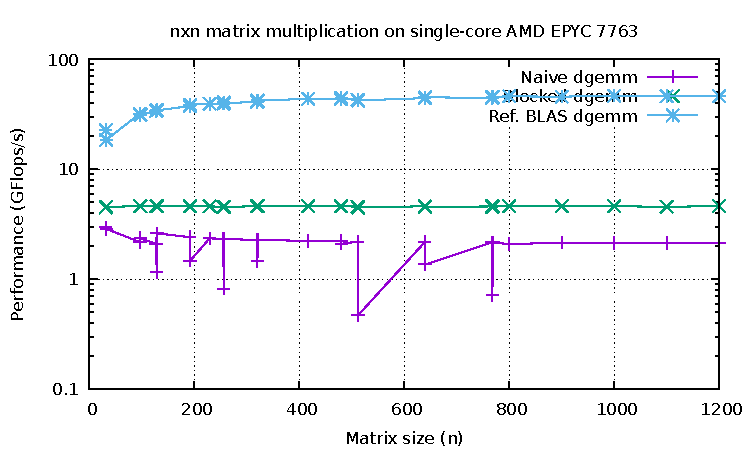
\includegraphics[width=0.8\textwidth]{../matrix_mult/timing_mavx2.pdf}
    \caption{Performance of the three algorithms using several compiler flags including mavx2 and pragma directives.}
\label{fig:performance_mavx2}
\end{figure}
Using the graph, we can analyze more quantitatively the performance of the three algorithms. We can see that 
the performance of the naive algorithm is significantly lower than the performance of the reference and blocked algorithms.
We didn't expect the blocked algorithm to perform better than the reference algorithm since the OpenBLAS library is
highly optimized for matrix-matrix multiplication. However, we can see that the performance of the blocked algorithm
performed significantly better than the naive algorithm and doesn't suffer from dips in performance as the size of the 
matrix increases. This is due to the blocked algorithm's ability to utilize the cache more effectively and reduce the
number of cache misses. We tried extending the blocked matrix algorithm to include the L2 chache using the same 
logic and structure but failed in the implementation.
% Bonus (20 points): Employ any advanced techniques from library implementations as described
% in the references provided in the motivation Section 4.1, including any references therein or other
% relevant resource. However, remember to accurately cite all your sources
Looking back at the original implementation of the blocked algorithm, we can see that its performance improved significantly
by using the optimization flags and pragma directives. The final result of 11.68\% shows a 852\% improvement over the first
block algorithm implementation.



\bibliographystyle{plain}
\bibliography{refs} % Entries are in the refs.bib file

\subsection*{Appendix}
I apologize for the inconvenience of the image sizes and the orientation. The output of the image
was given by the software, and I had to rotate them to fit the page and become most readable.

\begin{figure}[htbp]
    \centering
    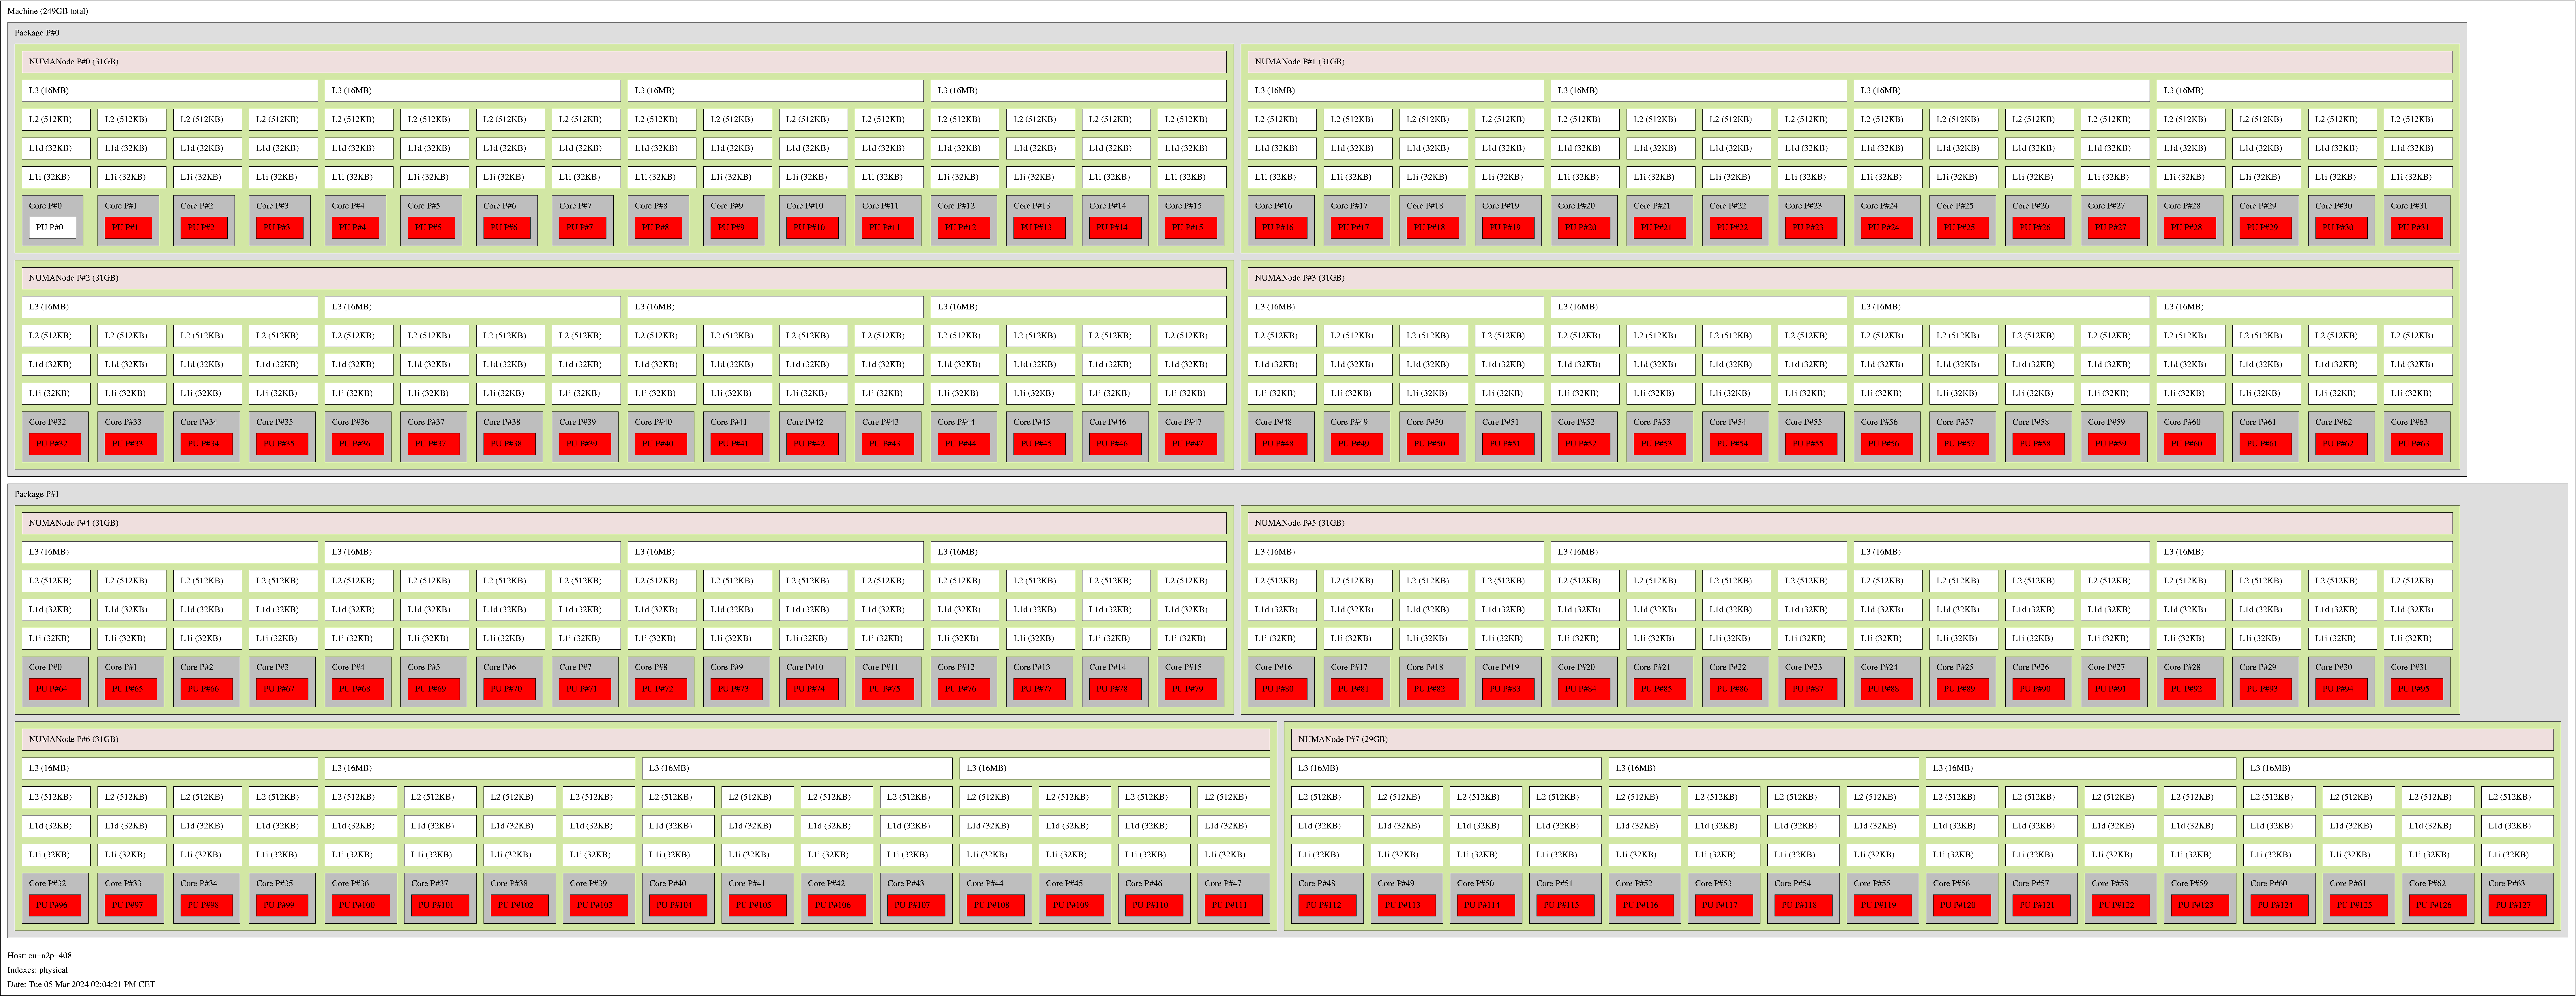
\includegraphics[width=1.5\textwidth, angle=90]{../cache_main_mem/eulerVII_I/EPYC_7H12.pdf}
    \caption{Memory Hierarchy of the AMD EPYC 7H12 Processor.}
\label{fig:7H12_processor}
\end{figure}


\begin{figure}[htbp]
    \centering
    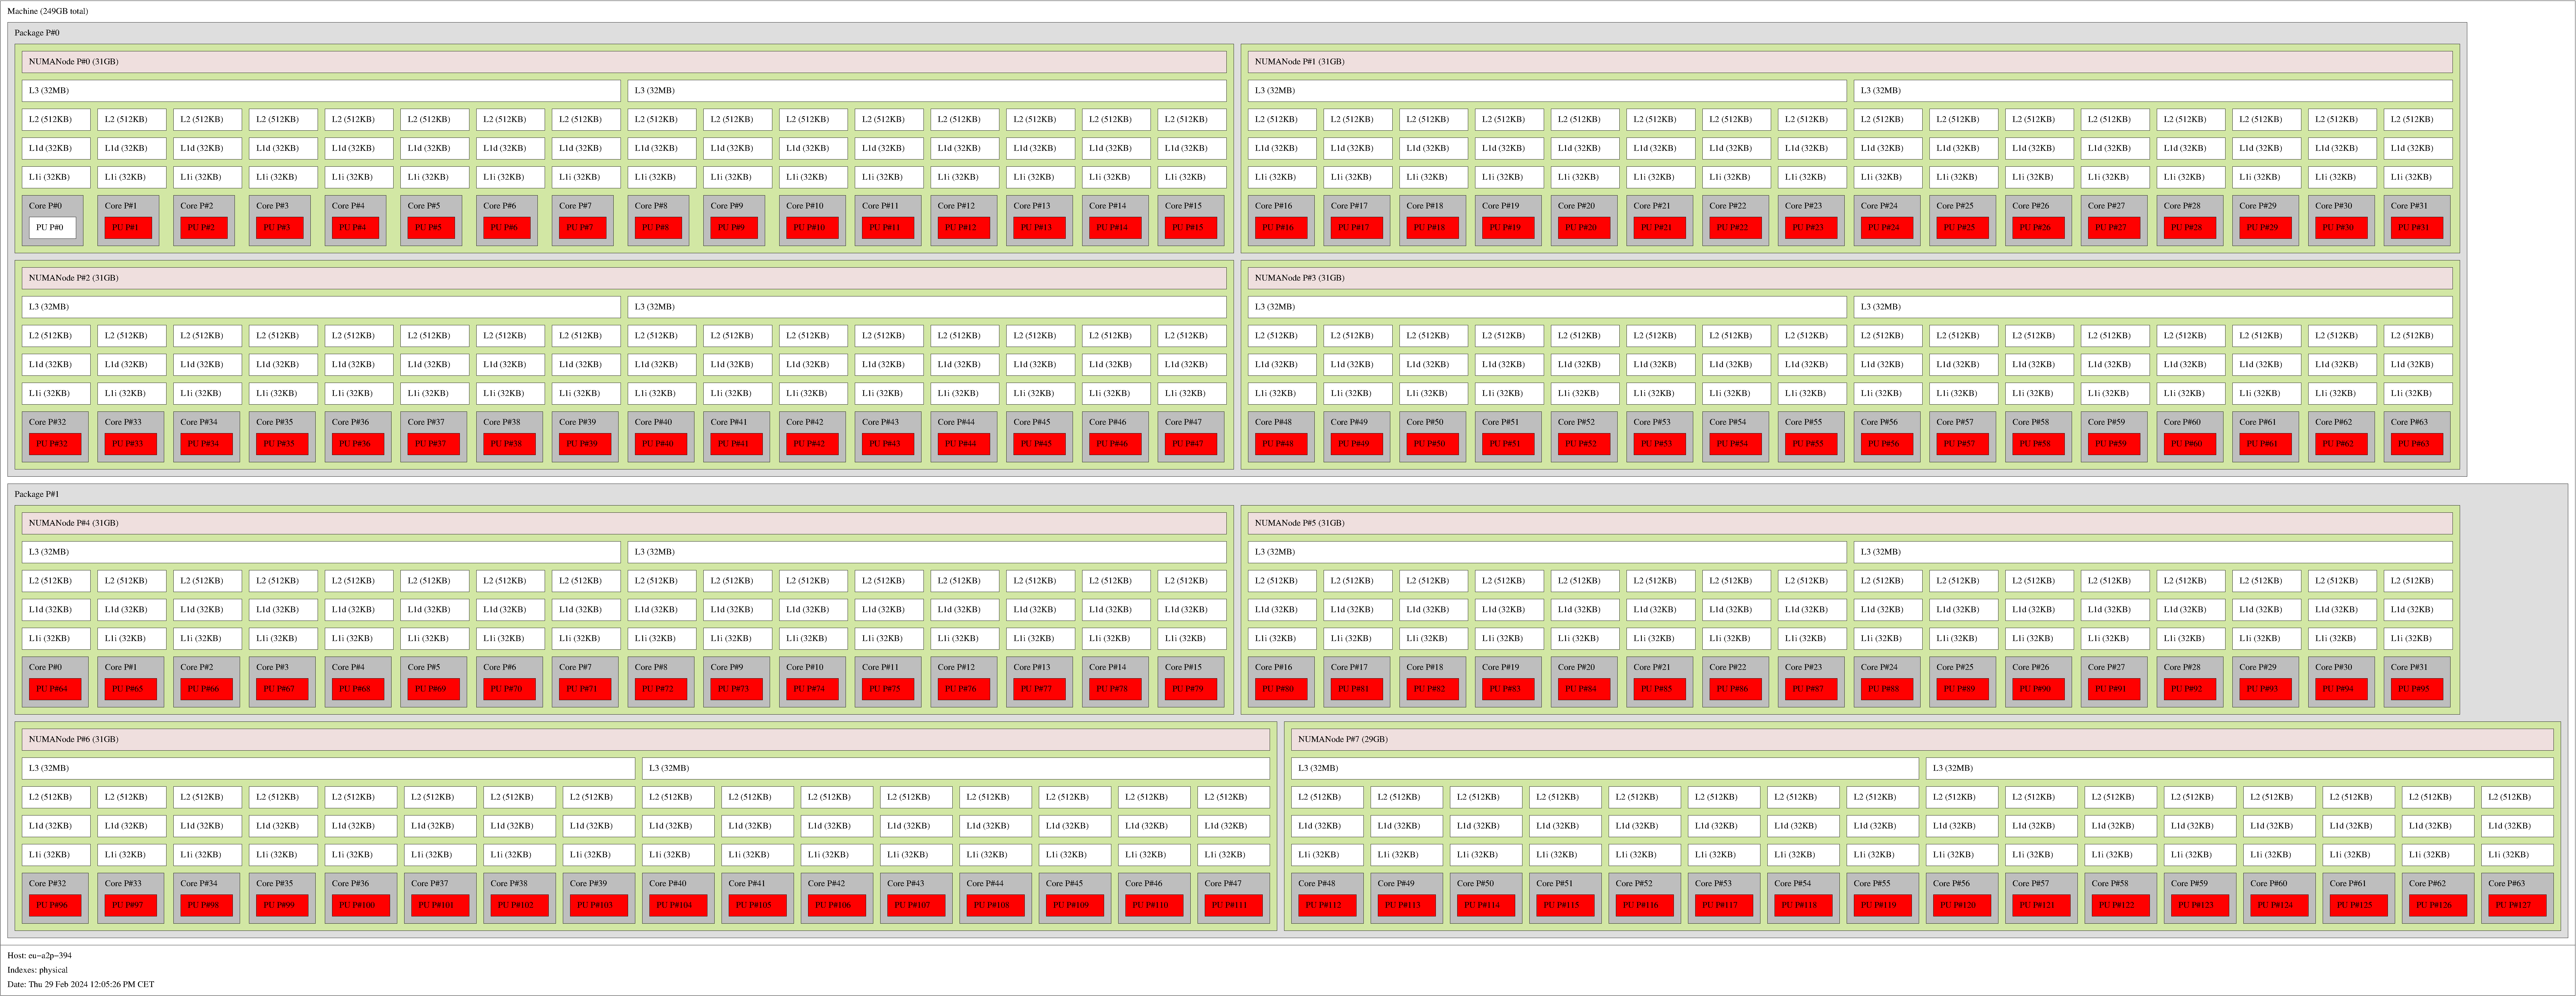
\includegraphics[width=1.5\textwidth, angle=90]{../cache_main_mem/EulerVII_II/EPYC_7763.pdf}
    \caption{Memory Hierarchy of the AMD EPYC 7763 Processor.}
\label{fig:7763_processor}
\end{figure}

\end{document}
